\begin{frame}[fragile]
  \frametitle{Clases y objetos}
  
  Una clase no es m\'as que una plantilla gen\'erica a partir de la cual se pueden instanciar objetos;
  en esta plantilla es donde se definen qu\'e atributos y m\'etodos tendr\'an los objetos de esa clase.
  
  \begin{figure}
    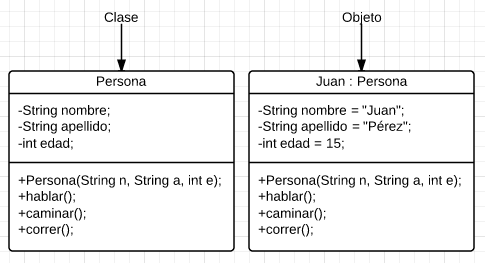
\includegraphics[width=0.6\textwidth]{Imagenes/ClaseObjeto.jpg}
    % \caption{\label{fig:Ejm}Esta funci\'on imprime los dos parametros ingresados.}
  \end{figure}
  
\end{frame}

